\newpage
\chapter{\normalfont Market Efficiency}
With econ, there are so many assumptions that have to be made. When we do any analysis of markets, its important to remember the assumptions to avoid silly mistakes. 
\textbf{Market Assumptions}
\begin{itemize}
    \item The market is perfectly competitive
        \begin{itemize}
            \item There exists many buyers and sellers
        \end{itemize}
    \item Consumers are rational
        \begin{itemize}
            \item They will maximize utility
        \end{itemize}
    \item Producers are rational
        \begin{itemize}
            \item They will act in their interest to maximize profit
        \end{itemize}
    \item No government intervention
        \begin{itemize}
            \item No taxes, subsidies, etc
        \end{itemize}
    \item No externalities
        \begin{itemize}
            \item No additional costs or benefits to people not directly invokved in the transaction
            \item MPB = MSB and MPC = MSC
        \end{itemize}
\end{itemize}
\lecture{7}{thur 23 sep 8:35}{Resources}
\section{Allocating Resources}

Consumers often have to make \textbf{Marginal Decisions} behind their purchases, and its something that economists take into consideration. The big idea behind marginal decision making is that \textbf{Marginal Utility = Marginal Cost}. You can see Marginal Utility written as Marginal Benefit, but they are interchangeable.
\begin{definition}
    Marginal Decision is the added "satisfaction" from consuming another unit vs. the cost of the additional unit. Marginal is usually used to represent the "additional". Marginal utility is the utilty from each additional unit. Marginal cost is the cost of each additional unit.
\end{definition}

With this comes the idea of \textbf{Diminishing Marginal Utility:} each additional unit will bring less benefit to the consumer than the previous unit. This means that rational consumers will purchase in order to maximize their marginal utility, or their "happiness". There are multiple different ways to maximize your resources which is Allocative and Productive Efficiency.

\begin{description}
    \item[Allocative Efficiency] Consumers who value good/service at least as much as it cost to produce are able to buy it. HIgh value consumers are able to obtain the goods or services. MB = MC
    \item[Productive Efficiency] All producers who are able to produce their good/services at the price in the market or below are able to sell their items. Goods and services produced at lowest possible cost. MC = MB
\end{description}

With market efficency, comes the idea of surplus. There are a few types of surplus that you should know, stuch as \textbf{Consumer Surplus (CS)}, \textbf{Producer Surplus (PS)}, and \textbf{Total Surplus (TS)}.
\begin{description}
    \item[Consumer Surplus] The difference between what consumers are willing to pay and have to pay ($P_m$)
    \item[Producer Surplus] The difference between the price at which producers would be willing to sell and what they can charge ($P_m$)
    \item[Total Surplus] CS + PS, and is maximised in perfectly competitive markets at equilibrium
\end{description}
Make sure to remember that if you are trying to find the regions on a graph, its usually in the shape of a triangle. So $\frac{1}{2}bh$ can find the area, and its always a \$ amount. 

\begin{definition}
    Deadweight Loss is missed opportunities to have mutually beneficial transactions, as it decreases total surplus and becomes inefficient. 
\end{definition}
\begin{itemize}
    \item[!] DWL is usually a side effect of government intervention, but could be caused by others.
\end{itemize}

Lets look at some examples of market efficiency, specifically at equilibrium and at disequilibrium. 

\begin{figure}[H]
\begin{center}
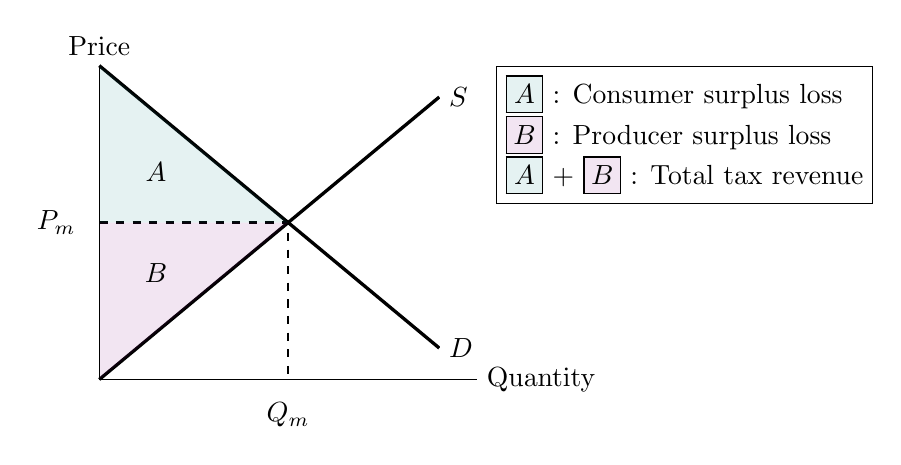
\begin{tikzpicture}
\begin{axis}[
scale=0.7,
xmin = 0, xmax = 10,
ymin = 0, ymax = 10, 
axis lines* = left,
xtick = \empty, ytick = \empty,
axis on top, 
clip = false,
]

\addplot[color = black, very thick] coordinates {(0,10) (9,1)};
\addplot[color = black, very thick] coordinates {(0,0) (9,9)};

\addplot[color = black, dashed, thick] coordinates {(0,5) (5,5) (5,0)};

% Fill
\fill[teal, opacity = 0.1] (0,10) -- (5,5) -- (0,5);
\fill[violet, opacity = 0.1] (0,0) -- (5,5) -- (0,5);

\node [right] at (current axis.right of origin) {Quantity};
\node [above] at (current axis.above origin) {Price};
\node [left = 5pt] at (0,5) {$P_m$};
\node [below = 5pt] at (5,0) {$Q_m$};
\node [right, fill = white] at (9,1) {$D$};
\node [right, fill = white] at (9,9) {$S$};
\node [above] at (1.5, 6) {$A$};
\node [below] at (1.5, 4) {$B$};
\node [below right, draw, align = left] at (10.5, 10) {
\fcolorbox{black}{teal!10}{\makebox[\fontcharht\font`X]{$A$}} : Consumer surplus loss \\
\fcolorbox{black}{violet!10}{\makebox[\fontcharht\font`X]{$B$}} : Producer surplus loss \\
\fcolorbox{black}{teal!10}{\makebox[\fontcharht\font`X]{$A$}} + \fcolorbox{black}{violet!10}{\makebox[\fontcharht\font`X]{$B$}} : Total tax revenue
};
\end{axis}
\end{tikzpicture}
\caption{Market for NYC Apartments}
\label{fig:nyc}
\end{center}
\end{figure}

\ref{fig:nyc} represents a market at equilibrium, where Total Surplus is maximized, and DWL is no where to exist. Now if we were to graph the market in disequilibrium, it would look a bit different.

\begin{figure}[h!]
\begin{center}
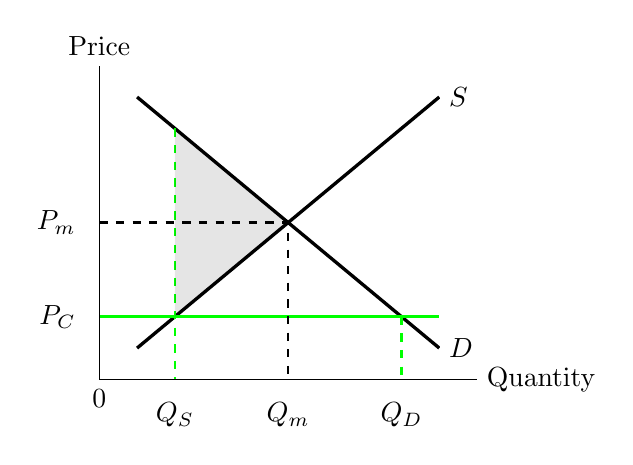
\begin{tikzpicture}
\begin{axis}[
scale=0.7,
xmin = 0, xmax = 10,
ymin = 0, ymax = 10, 
axis lines* = left,
xtick = {0}, ytick = \empty,
axis on top, 
clip = false,
]

\addplot[color = black, very thick] coordinates {(1,9) (9,1)};
\addplot[color = black, very thick] coordinates {(1,1) (9,9)};
\addplot[color = green, very thick] coordinates {(0,2) (9,2)};

\addplot[color = black, dashed, thick] coordinates {(0,5) (5,5) (5,0)};
\addplot[color = green, dashed, thick] coordinates {(2,8) (2,0)};
\addplot[color = green, dashed, thick] coordinates {(8,2) (8,0)};

\fill[black, opacity = 0.1] (2,8) -- (5,5) -- (2,2);

\node [right] at (current axis.right of origin) {Quantity};
\node [above] at (current axis.above origin) {Price};
\node [left = 5pt] at (0,5) {$P_m$};
\node [below = 5pt] at (5,0) {$Q_m$};
\node [right, fill = white] at (9,1) {$D$};
\node [right, fill = white] at (9,9) {$S$};
\node [below = 5pt] at (2,0) {$Q_S$};
\node [below = 5pt] at (8,0) {$Q_D$};
\node [left = 5pt] at (0,2) {$P_C$};
\end{axis}
\end{tikzpicture}
\caption{Market for NYC Apartments, with rent control}
\label{fig:nyc2}
\end{center}
\end{figure}

\ref{fig:nyc2} represents a market at disequilibrium due to a price ceiling that was placed on apartments in NYC. We will cover floors and ceilings later, but for now just understand that it prevents prices of apartments from rising above the line. This causes DWL in the black region, where both CS and PS, and in turn TS, is lost. 
